\begin{frame}
    \frametitle{Ambulance blockage problem in UK}
    \centering

    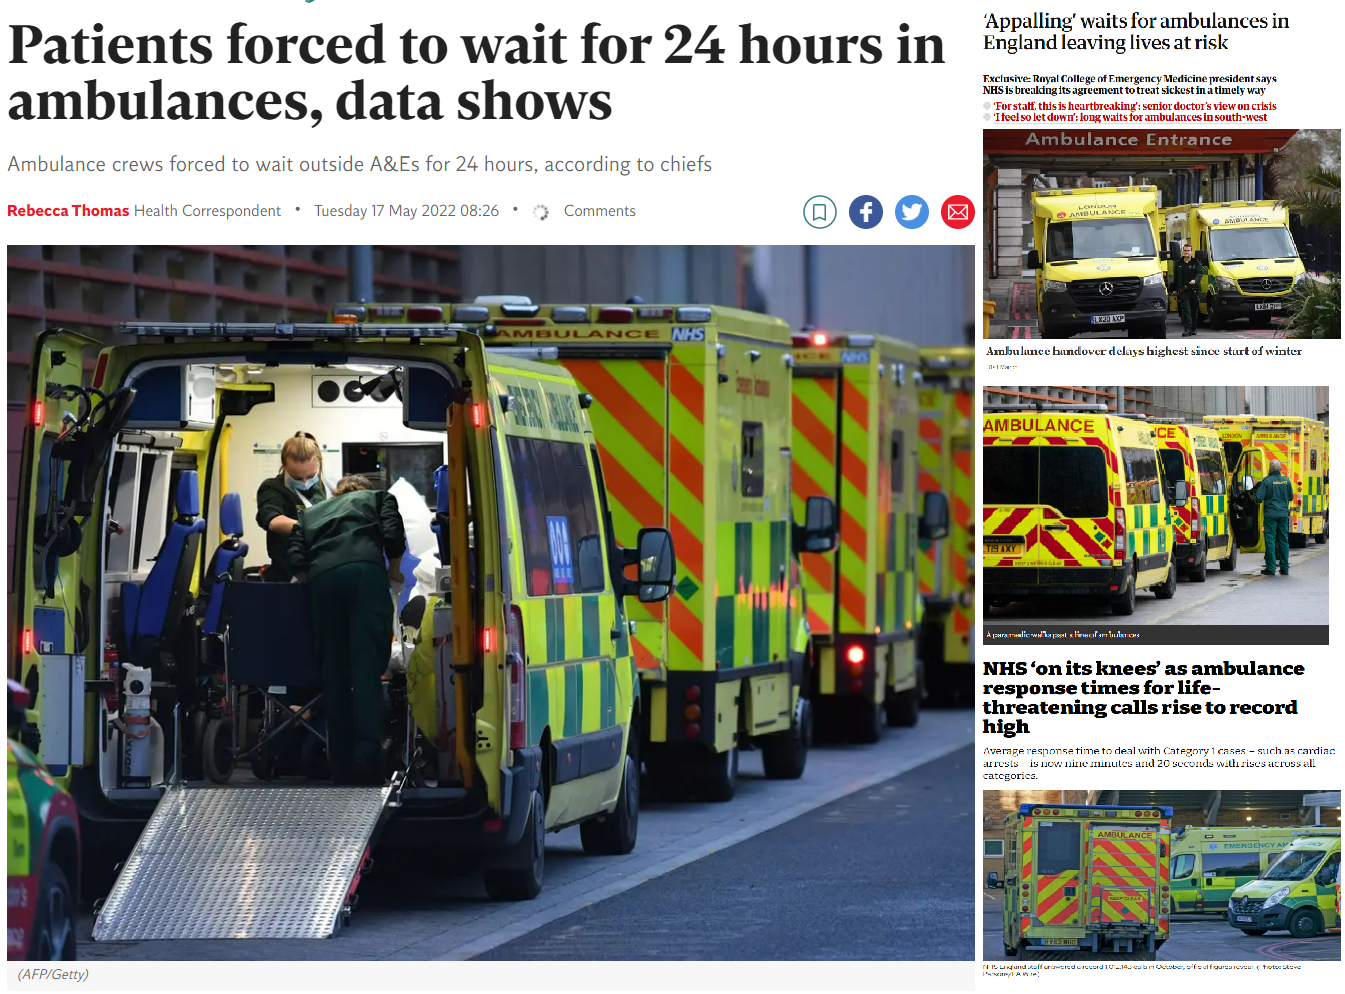
\includegraphics[scale=0.3]{Bin/ambulance_pics/articles.PNG}
        
\end{frame}



\begin{frame}
    \Huge
    \centering

    \textbf{Queueing theory}

    \(\times\)

    \textbf{Game theory}
    
\end{frame}

\begin{frame}
    \frametitle{Queueing representation of hospital}
    \centering
    \begin{figure}[h]
        \centering
        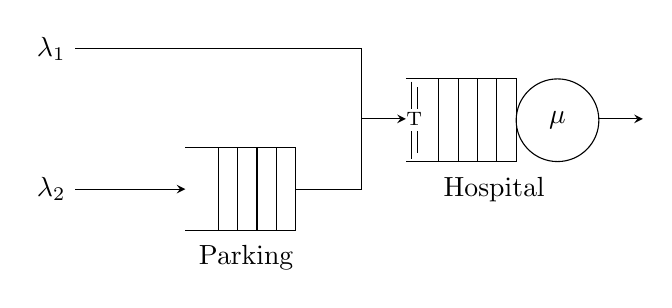
\begin{tikzpicture}[>=stealth, scale=0.7] %arrow type
            % Queue 1
            \draw (1,0) -- ++(2cm,0) -- ++(0,-1.5cm) -- ++(-2cm,0);
            \foreach \i in {1,...,4}
            \draw (3cm-\i*10pt,0) -- +(0,-1.5cm);

            % Queue 2
            \draw (5,1.25) -- ++(2cm,0) -- ++(0,-1.5cm) -- ++(-2cm,0);
            \foreach \i in {1,...,4}
            \draw (7cm-\i*10pt,1.25) -- +(0,-1.5cm);
            \draw (7.75,0.5) circle [radius=0.75cm];
            \node at (7.75, 0.5) {\(\mu\)};

            % The two vertical lines at the very start of Queue 2
            \draw (7cm-54pt,1.2) -- +(0,-0.5cm);
            \draw (7cm-54pt,0.3) -- +(0,-0.5cm);
            \draw (7cm-51pt,1.1) -- +(0,-0.4cm);
            \draw (7cm-51pt,0.3) -- +(0,-0.4cm);
            \node[anchor=north] at (5.15, 0.83 cm) {\scriptsize{T}};

            % the arrows and labels (Queue 1+2)
            \node[align=center] at (1cm,-2cm) {};
            \node[align=center] at (6cm,-0.75cm) {};

            % Arrows lines
            \draw (4.2, 1.8) -- +(-5.2,0) node[left] {\( \lambda_1 \)};
            \draw[<-] (1,-0.75) -- +(-2,0) node[left] {\( \lambda_2 \)};
            \draw[->] (4.2, 0.525) -- (5, 0.525);
            \draw[->] (8.5,0.525) -- (9.3,0.525);

            % Parking and Hospital Labels
            \node[align=center] at (2.1cm,-2cm) {Parking};
            \node[align=center] at (6.6cm,-0.75cm) {Hospital};

            % Others lines
            \draw[-] (3,-0.75) -- (4.2,-0.75);
            \draw (4.2, 0.525) -- (4.2, -0.75);
            \draw (4.2, 1.8) -- (4.2, 0.525);

        \end{tikzpicture}
    \end{figure}

    \small
    \begin{itemize}
        \item \( \lambda_1 \): Arrival rate of non-ambulance patients
        \item \( \lambda_2 \): Arrival rate of ambulance patients
        \item \( \mu \): Service rate
        \item \( T \): Threshold
    \end{itemize}
\end{frame}



\begin{frame}
    \frametitle{The game}
    \centering
    
\includegraphics[scale=0.1]{Bin/cartoon_pics/ambulance_cartoon.png}

    \vspace{0.5cm}
    
\begin{tikzpicture}
        \draw[->, ultra thick] (-0.5, 0) -- ++(-1.5, -2);
        \draw[->, ultra thick] (0.5, 0) -- ++(1.5, -2);
    \end{tikzpicture}

    \vspace{0.5cm}
    
\includegraphics[scale=0.1]{Bin/cartoon_pics/hospital.png}
    \hspace{3cm}
    
\includegraphics[scale=0.1]{Bin/cartoon_pics/hospital.png}

\end{frame}


\begin{frame}
    \frametitle{Players - Strategies - Objectives}
    \centering

    
\includegraphics[scale=0.1]{Bin/cartoon_pics/ambulance_cartoon.png}
    \hspace{2cm}
    
\includegraphics[scale=0.1]{Bin/cartoon_pics/hospital.png}
    \hspace{2cm}
    
\includegraphics[scale=0.1]{Bin/cartoon_pics/hospital.png}

    \vspace{1cm}
    
\includegraphics[scale=0.2]{Bin/cartoon_pics/arrows.png}
    \hspace{2cm}
    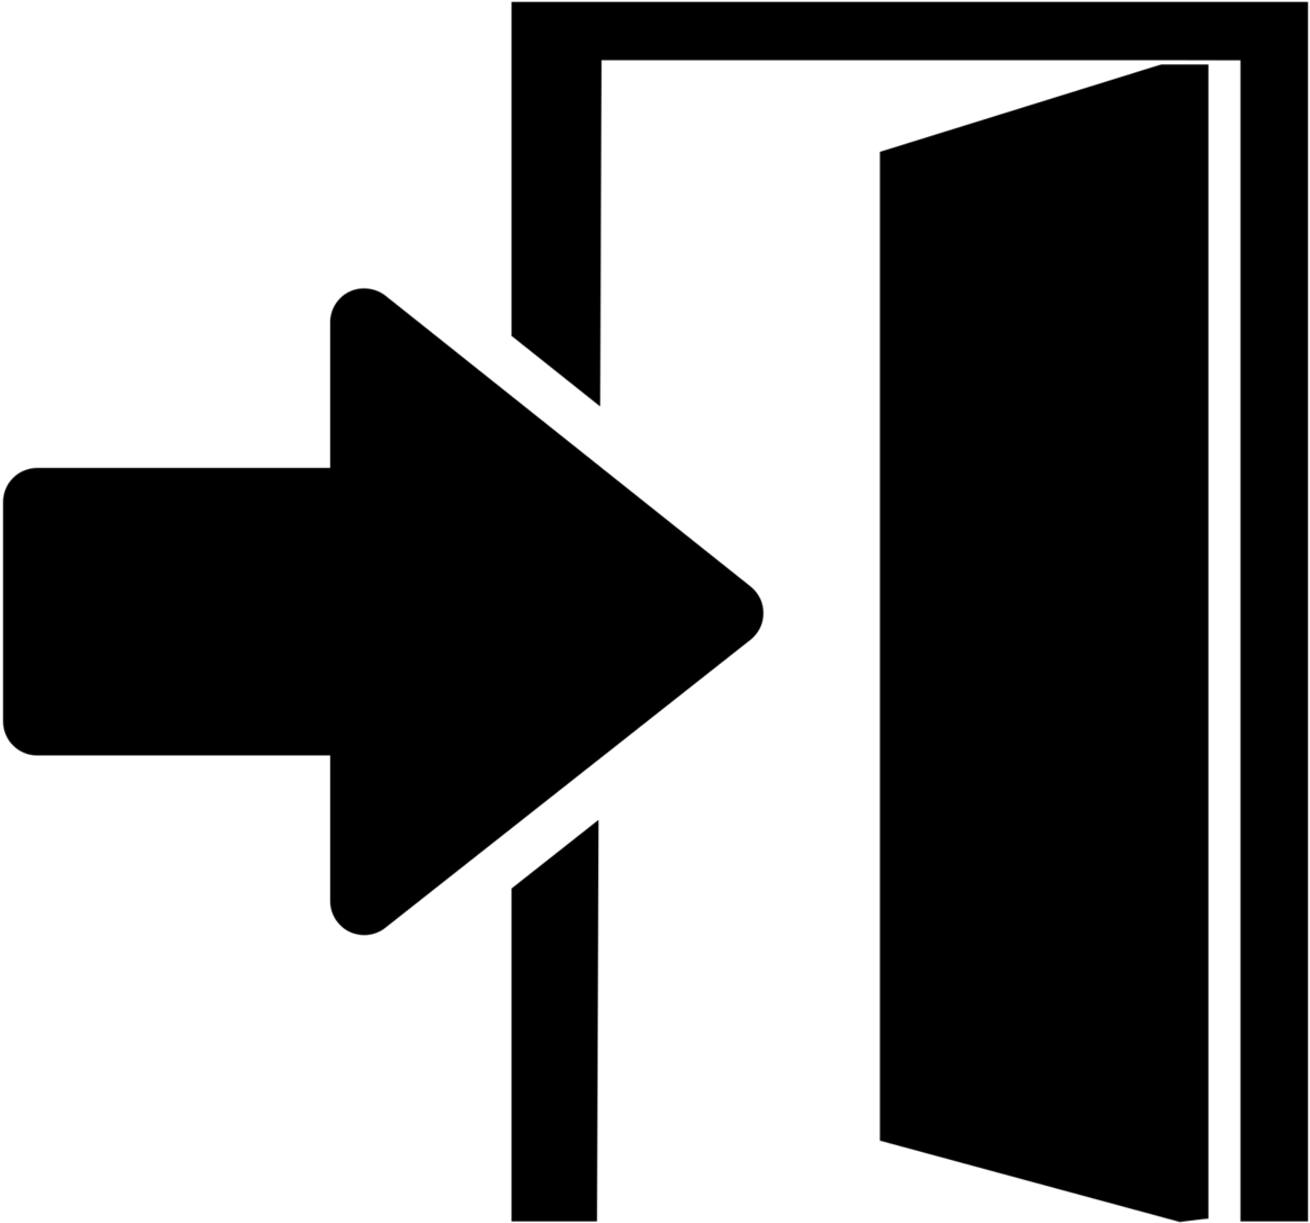
\includegraphics[scale=0.04]{Bin/cartoon_pics/door.png}
    \hspace{2cm}
    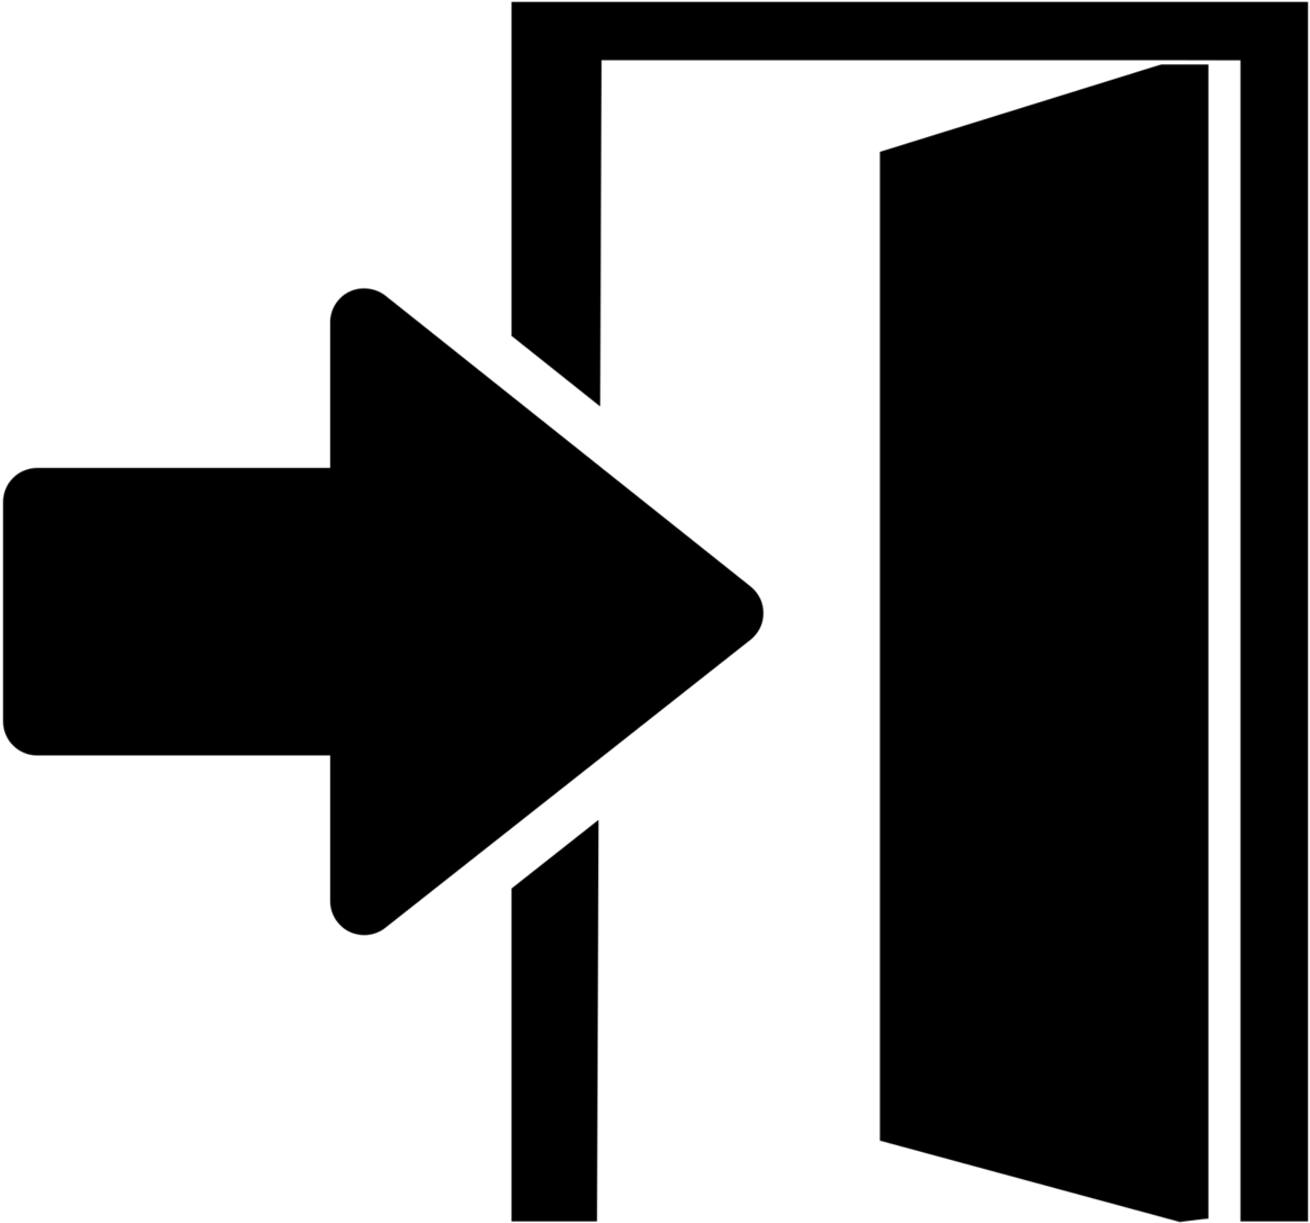
\includegraphics[scale=0.04]{Bin/cartoon_pics/door.png}

    \(p_A, p_B \in [0, 1] \hspace{2cm} T_A \in [1, N_A] 
    \hspace{2cm} T_B \in [1, N_B]\)
    \(p_A + p_B = 1 \hspace{8cm}\)
    
    \vspace{1cm}
    \small
    \(
        \qquad \min \bar{B} \hspace{2.4cm} P(W^{(A)} < t) > 0.95 
        \hspace{0.7cm} P(W^{(B)} < t) > 0.95
    \)
\end{frame}


% \begin{frame}
%     \frametitle{Imperfect information extensive form game}
%     \centering

%     \begin{figure}[ht]
%         \centering
%         \begin{tikzpicture}[-, node distance = 2cm, scale=0.75, auto, rotate=90, transform shape]

%             \only<2>{
%                 \draw[thick] (-3, 0) -- (3, 0) -- (3, -8) -- (-3, -8) -- (-3, 0);
%             }

%             \node[anchor=north, rotate=270] (QA) at (0.3,-0.3) {\(H_A\)};
%             \node[anchor=north](QA_d1) at (-2.5, -3) {};
%             \node[anchor=north](QA_d2) at (-1, -3) {};
%             \node[anchor=north](QA_d3) at (0.5, -2) {\(\dots\)};
%             \node[anchor=north](QA_d4) at (2.5, -3) {};
        
%             \path[->] (QA) edge node [above, rotate=180+50] {\scriptsize{\(T_A=1\)}}(QA_d1);
%             \path[->] (QA) edge node [above, rotate=180+70] {\scriptsize{\(T_A=2\)}}(QA_d2);
%             \path[<-] (QA_d4) edge node [above, rotate=310] {\scriptsize{\(T_A = N_A\)}}(QA);
        
%             \path (QA_d1) [dashed] edge node {}(QA_d4);
%             \path (QA_d1) [bend right] edge node {}(QA_d4);
        
%             \node[anchor=north, rotate=270](QB) at (0.3, -4.3) {\(H_B\)};
%             \node[anchor=north](QB_d1) at (-2.5, -7) {};
%             \node[anchor=north](QB_d2) at (-1, -7) {};
%             \node[anchor=north](QB_d3) at (0.5, -6) {\(\dots\)};
%             \node[anchor=north](QB_d4) at (2.5, -7) {};
        
%             \path[->] (QB) edge node [above, rotate=180+50] {\scriptsize{\(T_B=1\)}}(QB_d1);
%             \path[->] (QB) edge node [above, rotate=180+70] {\scriptsize{\(T_B=2\)}}(QB_d2);
%             \path[<-] (QB_d4) edge node [above, rotate=310] {\scriptsize{\(T_B = N_B\)}}(QB);
        
%             \path (QB_d1) [bend right] edge node {}(QB_d4);
        
%             \node[anchor=north, rotate=270] (D) at (0.3, -8.3) {\(A\)};
%             \node[anchor=north, rotate=270](D_d1) at (-2.5, -11) {};
%             \node[anchor=north](D_dots) at (0, -10) {\(\dots\)};
%             \node[anchor=north, rotate=270](D_d2) at (2.5, -11) {};
        
%             \path[->] (D) edge node [below, rotate=180+43] {\scriptsize{\(p_A=0\)}}(D_d1);
%             \path[<-] (D_d2) edge node [above, rotate=310] {\scriptsize{\(p_A=1\)}}(D);
        
%             \path (D_d1) [bend right] edge node {}(D_d2);
        
%         \end{tikzpicture}        
%     \end{figure}
% \end{frame}

% \begin{frame}
%     \frametitle{Hospital's utility}

%     \begin{equation*}
%         U_{T_A,T_B}^{(i)} = 1 - \left[ (P(W^{(i)} < t) - 0.95)^2 \right]
%     \end{equation*}

%     \scriptsize
%     \begin{equation*}
%         A = 
%         \begin{pmatrix}
%             U_{1,1}^A & U_{1,2}^A & \dots & U_{1,N_B}^A \\ 
%             U_{2,1}^A & U_{2,2}^A & \dots & U_{2,N_B}^A \\
%             \vdots & \vdots & \ddots & \vdots \\
%             U_{N_A,1}^A & U_{N_A,2}^A & \dots & U_{N_A,N_B}^A \\
%         \end{pmatrix}, \quad
%         B = 
%         \begin{pmatrix}
%             U_{1,1}^B & U_{1,2}^B & \dots & U_{1,N_B}^B \\ 
%             U_{2,1}^B & U_{2,2}^B & \dots & U_{2,N_B}^B \\
%             \vdots & \vdots & \ddots & \vdots \\
%             U_{N_A,1}^B & U_{N_A,2}^B & \dots & U_{N_A,N_B}^B \\
%         \end{pmatrix}
%     \end{equation*}

% \end{frame}


% \begin{frame}
%     \frametitle{Nash Equilibrium}
%     \centering

%     \small
%     \begin{equation*}
%         A = 
%         \begin{pmatrix}
%             8.39 & 8.39 & 8.39 & 8.39 \\
%             8.96 & 8.85 & 8.65 & 8.45 \\
%             9.95 & 9.87 & 9.6  & 9.2  \\
%             4.37 & 5.11 & 8.6  & 9.91 \\
%         \end{pmatrix} \qquad
%         B = 
%         \begin{pmatrix}
%             8.39 & 8.96 & 9.95 & 4.37 \\
%             8.39 & 8.85 & 9.87 & 5.11 \\
%             8.39 & 8.65 & 9.6 &  8.6 \\ 
%             8.39 & 8.45 & 9.2 &  9.91 \\
%         \end{pmatrix}
%     \end{equation*}

%     \vspace{1cm}

%     \begin{equation*}
%         \textbf{Nash Equilibria: } \quad
%         \begin{array}{c|c}
%             \underline{\quad A \quad} & \underline{\quad B \quad} \\
%             (0, 0, 1, 0) & (0, 0, 1, 0) \\ 
%             \hline
%             (0, 0, 0, 1) & (0, 0, 0, 1) \\ 
%             \hline
%             (0, 0, 0.4, 0.6) & (0, 0, 0.4, 0.6) \\
%         \end{array}
%     \end{equation*}
% \end{frame}


\begin{frame}
    \huge
    \centering

    \textbf{Evolutionary Game Theory}
    

\end{frame}

\begin{frame}
    \frametitle{Asymmetric replicator dynamics - \(t = 1.5\)}
    \begin{columns}
        \centering
        \column{\dimexpr\paperwidth-10pt}
        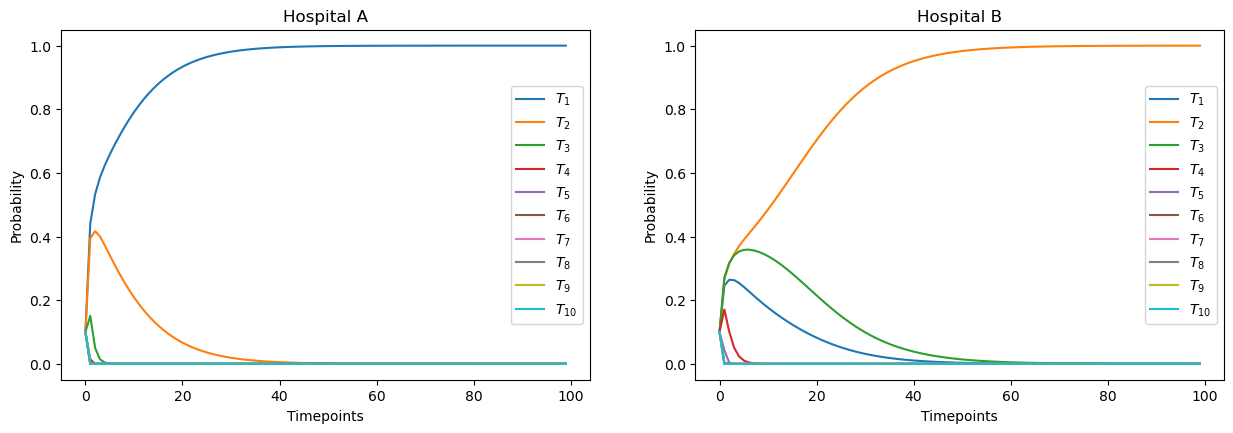
\includegraphics[width=\textwidth]{Bin/replicator_dynamics/ard_t_1.5.png}

        \[T_A = 1  \qquad \qquad \qquad \qquad \qquad \qquad T_B = 2\]
    \end{columns}

\end{frame}


\begin{frame}
    \frametitle{Asymmetric replicator dynamics - \(t = 1.7\)}

    \begin{columns}
        \centering
        \column{\dimexpr\paperwidth-10pt}
        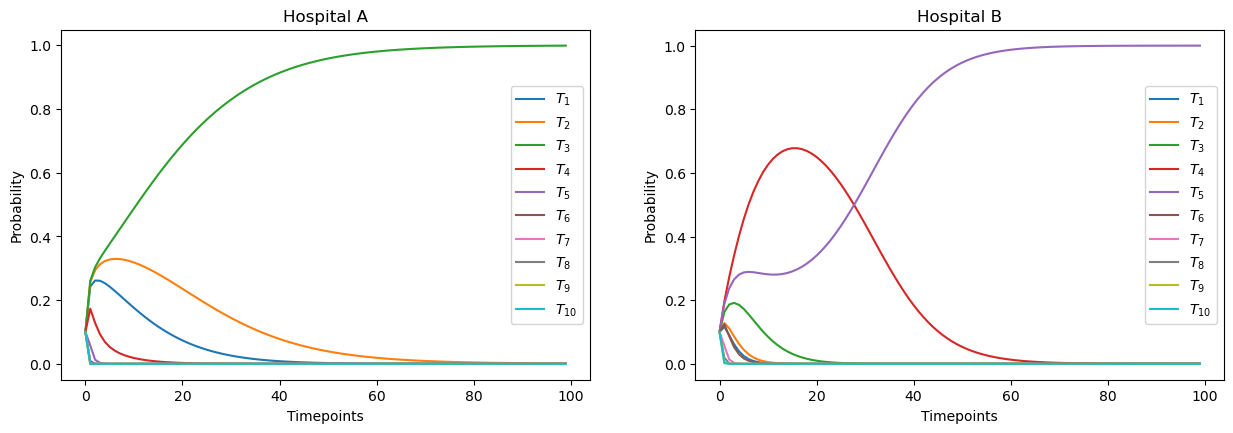
\includegraphics[width=\textwidth]{Bin/replicator_dynamics/ard_t_1.7.png}

        \[T_A = 3  \qquad \qquad \qquad \qquad \qquad \qquad T_B = 5\]
    \end{columns}
    
\end{frame}


\begin{frame}
    \frametitle{Asymmetric replicator dynamics - \(t = 2\)}

    \begin{columns}
        \centering
        \column{\dimexpr\paperwidth-10pt}
        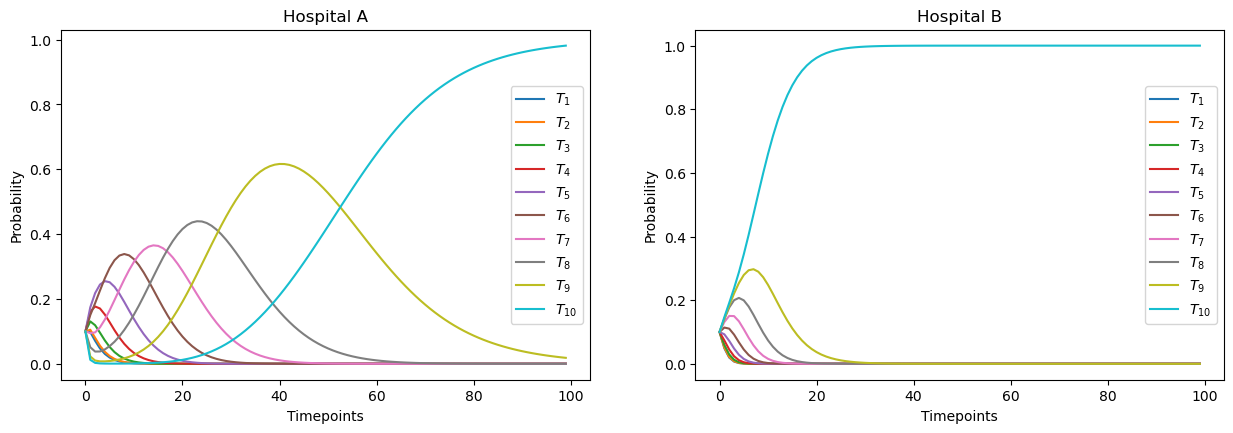
\includegraphics[width=\textwidth]{Bin/replicator_dynamics/ard_t_2.png}

        \[ T_A = 10  \qquad \qquad \qquad \qquad \qquad \qquad T_B = 10\]
    \end{columns}
    
\end{frame}

\begin{frame}
    \frametitle{Asymmetric replicator dynamics - Incentives}
    \centering

    % 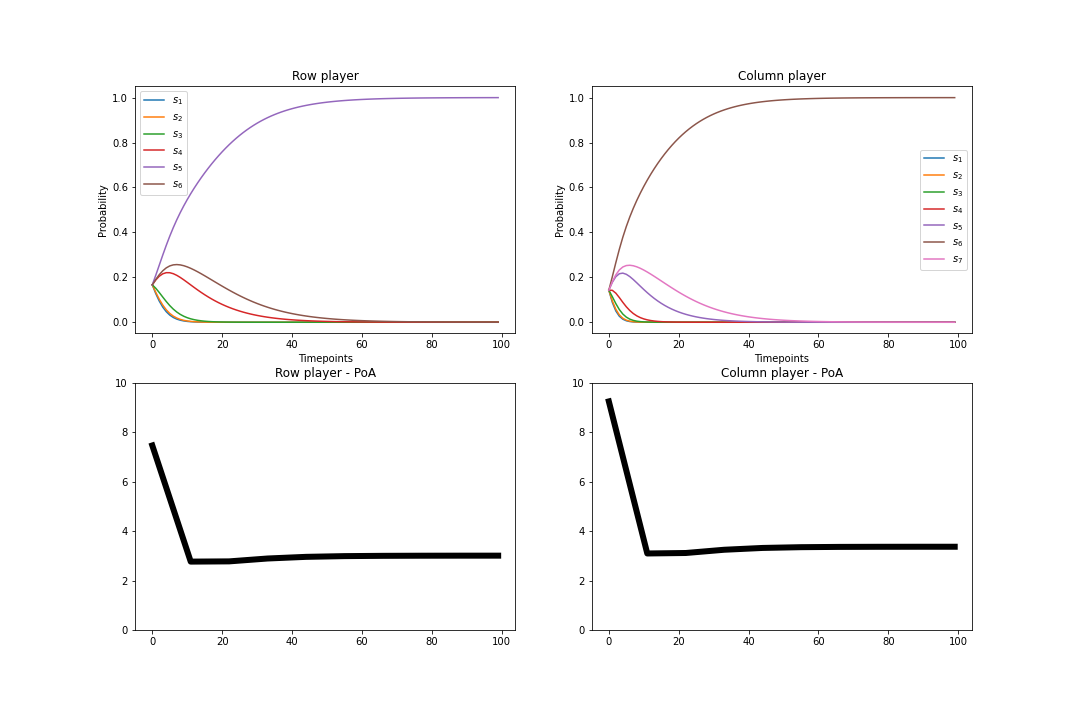
\includegraphics[width=\textwidth, trim = 90 367 90 70, clip]{Bin/replicator_dynamics/ARD_game.png}
    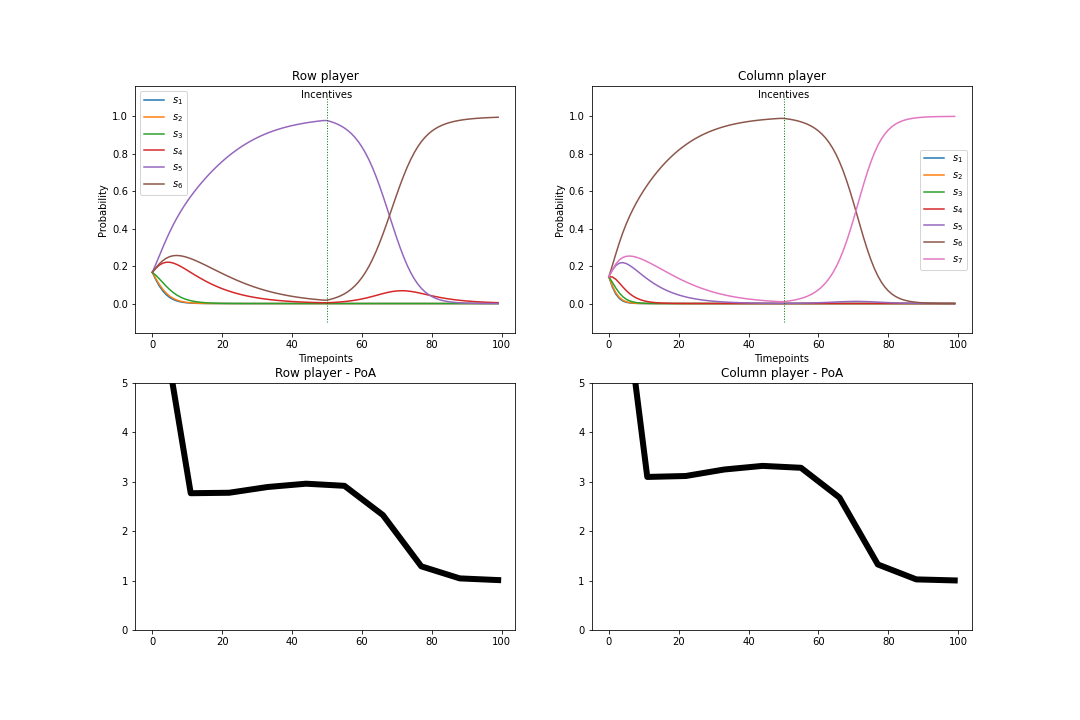
\includegraphics[width=\textwidth, trim = 90 367 90 70, clip]{Bin/replicator_dynamics/ARD_penalty_game.png}

    \[ T_A = 5  \rightarrow T_A = 6 \qquad \qquad \qquad T_B = 6 \rightarrow T_B = 7\]


    

\end{frame}

